\documentclass[]{article}
\usepackage{lmodern}
\usepackage{amssymb,amsmath}
\usepackage{ifxetex,ifluatex}
\usepackage{fixltx2e} % provides \textsubscript
\ifnum 0\ifxetex 1\fi\ifluatex 1\fi=0 % if pdftex
  \usepackage[T1]{fontenc}
  \usepackage[utf8]{inputenc}
\else % if luatex or xelatex
  \ifxetex
    \usepackage{mathspec}
  \else
    \usepackage{fontspec}
  \fi
  \defaultfontfeatures{Ligatures=TeX,Scale=MatchLowercase}
\fi
% use upquote if available, for straight quotes in verbatim environments
\IfFileExists{upquote.sty}{\usepackage{upquote}}{}
% use microtype if available
\IfFileExists{microtype.sty}{%
\usepackage{microtype}
\UseMicrotypeSet[protrusion]{basicmath} % disable protrusion for tt fonts
}{}
\usepackage[margin=1in]{geometry}
\usepackage{hyperref}
\hypersetup{unicode=true,
            pdftitle={R Notebook: Getting Dirty with Data},
            pdfborder={0 0 0},
            breaklinks=true}
\urlstyle{same}  % don't use monospace font for urls
\usepackage{color}
\usepackage{fancyvrb}
\newcommand{\VerbBar}{|}
\newcommand{\VERB}{\Verb[commandchars=\\\{\}]}
\DefineVerbatimEnvironment{Highlighting}{Verbatim}{commandchars=\\\{\}}
% Add ',fontsize=\small' for more characters per line
\usepackage{framed}
\definecolor{shadecolor}{RGB}{248,248,248}
\newenvironment{Shaded}{\begin{snugshade}}{\end{snugshade}}
\newcommand{\KeywordTok}[1]{\textcolor[rgb]{0.13,0.29,0.53}{\textbf{{#1}}}}
\newcommand{\DataTypeTok}[1]{\textcolor[rgb]{0.13,0.29,0.53}{{#1}}}
\newcommand{\DecValTok}[1]{\textcolor[rgb]{0.00,0.00,0.81}{{#1}}}
\newcommand{\BaseNTok}[1]{\textcolor[rgb]{0.00,0.00,0.81}{{#1}}}
\newcommand{\FloatTok}[1]{\textcolor[rgb]{0.00,0.00,0.81}{{#1}}}
\newcommand{\ConstantTok}[1]{\textcolor[rgb]{0.00,0.00,0.00}{{#1}}}
\newcommand{\CharTok}[1]{\textcolor[rgb]{0.31,0.60,0.02}{{#1}}}
\newcommand{\SpecialCharTok}[1]{\textcolor[rgb]{0.00,0.00,0.00}{{#1}}}
\newcommand{\StringTok}[1]{\textcolor[rgb]{0.31,0.60,0.02}{{#1}}}
\newcommand{\VerbatimStringTok}[1]{\textcolor[rgb]{0.31,0.60,0.02}{{#1}}}
\newcommand{\SpecialStringTok}[1]{\textcolor[rgb]{0.31,0.60,0.02}{{#1}}}
\newcommand{\ImportTok}[1]{{#1}}
\newcommand{\CommentTok}[1]{\textcolor[rgb]{0.56,0.35,0.01}{\textit{{#1}}}}
\newcommand{\DocumentationTok}[1]{\textcolor[rgb]{0.56,0.35,0.01}{\textbf{\textit{{#1}}}}}
\newcommand{\AnnotationTok}[1]{\textcolor[rgb]{0.56,0.35,0.01}{\textbf{\textit{{#1}}}}}
\newcommand{\CommentVarTok}[1]{\textcolor[rgb]{0.56,0.35,0.01}{\textbf{\textit{{#1}}}}}
\newcommand{\OtherTok}[1]{\textcolor[rgb]{0.56,0.35,0.01}{{#1}}}
\newcommand{\FunctionTok}[1]{\textcolor[rgb]{0.00,0.00,0.00}{{#1}}}
\newcommand{\VariableTok}[1]{\textcolor[rgb]{0.00,0.00,0.00}{{#1}}}
\newcommand{\ControlFlowTok}[1]{\textcolor[rgb]{0.13,0.29,0.53}{\textbf{{#1}}}}
\newcommand{\OperatorTok}[1]{\textcolor[rgb]{0.81,0.36,0.00}{\textbf{{#1}}}}
\newcommand{\BuiltInTok}[1]{{#1}}
\newcommand{\ExtensionTok}[1]{{#1}}
\newcommand{\PreprocessorTok}[1]{\textcolor[rgb]{0.56,0.35,0.01}{\textit{{#1}}}}
\newcommand{\AttributeTok}[1]{\textcolor[rgb]{0.77,0.63,0.00}{{#1}}}
\newcommand{\RegionMarkerTok}[1]{{#1}}
\newcommand{\InformationTok}[1]{\textcolor[rgb]{0.56,0.35,0.01}{\textbf{\textit{{#1}}}}}
\newcommand{\WarningTok}[1]{\textcolor[rgb]{0.56,0.35,0.01}{\textbf{\textit{{#1}}}}}
\newcommand{\AlertTok}[1]{\textcolor[rgb]{0.94,0.16,0.16}{{#1}}}
\newcommand{\ErrorTok}[1]{\textcolor[rgb]{0.64,0.00,0.00}{\textbf{{#1}}}}
\newcommand{\NormalTok}[1]{{#1}}
\usepackage{longtable,booktabs}
\usepackage{graphicx,grffile}
\makeatletter
\def\maxwidth{\ifdim\Gin@nat@width>\linewidth\linewidth\else\Gin@nat@width\fi}
\def\maxheight{\ifdim\Gin@nat@height>\textheight\textheight\else\Gin@nat@height\fi}
\makeatother
% Scale images if necessary, so that they will not overflow the page
% margins by default, and it is still possible to overwrite the defaults
% using explicit options in \includegraphics[width, height, ...]{}
\setkeys{Gin}{width=\maxwidth,height=\maxheight,keepaspectratio}
\IfFileExists{parskip.sty}{%
\usepackage{parskip}
}{% else
\setlength{\parindent}{0pt}
\setlength{\parskip}{6pt plus 2pt minus 1pt}
}
\setlength{\emergencystretch}{3em}  % prevent overfull lines
\providecommand{\tightlist}{%
  \setlength{\itemsep}{0pt}\setlength{\parskip}{0pt}}
\setcounter{secnumdepth}{0}
% Redefines (sub)paragraphs to behave more like sections
\ifx\paragraph\undefined\else
\let\oldparagraph\paragraph
\renewcommand{\paragraph}[1]{\oldparagraph{#1}\mbox{}}
\fi
\ifx\subparagraph\undefined\else
\let\oldsubparagraph\subparagraph
\renewcommand{\subparagraph}[1]{\oldsubparagraph{#1}\mbox{}}
\fi

%%% Use protect on footnotes to avoid problems with footnotes in titles
\let\rmarkdownfootnote\footnote%
\def\footnote{\protect\rmarkdownfootnote}

%%% Change title format to be more compact
\usepackage{titling}

% Create subtitle command for use in maketitle
\newcommand{\subtitle}[1]{
  \posttitle{
    \begin{center}\large#1\end{center}
    }
}

\setlength{\droptitle}{-2em}

  \title{R Notebook: Getting Dirty with Data}
    \pretitle{\vspace{\droptitle}\centering\huge}
  \posttitle{\par}
    \author{}
    \preauthor{}\postauthor{}
    \date{}
    \predate{}\postdate{}
  

\begin{document}
\maketitle

\section{Goal today: Use R Markdown to investigate a data
question!}\label{goal-today-use-r-markdown-to-investigate-a-data-question}

These data are originally from Kaggle
(\url{https://www.kaggle.com/dorbicycle/world-foodfeed-production}).
Laurel Brehm has done some reformatting \& cleaning, \& has uploaded the
results to RLadies GitHub.

The data were collected from Food and Agriculture Organization of the
United Nations. We have production in 1000 tonnes of \emph{food} (=for
people) and \emph{feed} (=for animals), per country over years. There is
also data about the country location (latitude and longitude).

\subsection{Data Summary}\label{data-summary}

What do these data look like?

\begin{verbatim}
## Warning: package 'dplyr' was built under R version 3.4.4
\end{verbatim}

\begin{verbatim}
## 
## Attaching package: 'dplyr'
\end{verbatim}

\begin{verbatim}
## The following objects are masked from 'package:stats':
## 
##     filter, lag
\end{verbatim}

\begin{verbatim}
## The following objects are masked from 'package:base':
## 
##     intersect, setdiff, setequal, union
\end{verbatim}

\begin{verbatim}
## Warning: package 'ggplot2' was built under R version 3.4.4
\end{verbatim}

\begin{verbatim}
## Warning: package 'knitr' was built under R version 3.4.4
\end{verbatim}

\begin{verbatim}
## # A tibble: 6 x 13
##   Area.Abbreviation Area.Code Area  Item.Code Item    Element.Code Element
##   <fct>                 <int> <fct>     <int> <fct>          <int> <fct>  
## 1 AFG                       2 Afgh~      2511 Wheat ~         5142 Food   
## 2 AFG                       2 Afgh~      2805 Rice (~         5142 Food   
## 3 AFG                       2 Afgh~      2513 Barley~         5521 Feed   
## 4 AFG                       2 Afgh~      2513 Barley~         5142 Food   
## 5 AFG                       2 Afgh~      2514 Maize ~         5521 Feed   
## 6 AFG                       2 Afgh~      2514 Maize ~         5142 Food   
## # ... with 6 more variables: Unit <fct>, latitude <dbl>, longitude <dbl>,
## #   Year <int>, KTonnes <int>, Crop <fct>
\end{verbatim}

What are the countries? What are the crops \& food-stuffs?

\begin{verbatim}
##   [1] "Afghanistan"                              
##   [2] "Albania"                                  
##   [3] "Algeria"                                  
##   [4] "Angola"                                   
##   [5] "Antigua and Barbuda"                      
##   [6] "Argentina"                                
##   [7] "Armenia"                                  
##   [8] "Australia"                                
##   [9] "Austria"                                  
##  [10] "Azerbaijan"                               
##  [11] "Bahamas"                                  
##  [12] "Bangladesh"                               
##  [13] "Barbados"                                 
##  [14] "Belarus"                                  
##  [15] "Belgium"                                  
##  [16] "Belize"                                   
##  [17] "Benin"                                    
##  [18] "Bermuda"                                  
##  [19] "Bolivia (Plurinational State of)"         
##  [20] "Bosnia and Herzegovina"                   
##  [21] "Botswana"                                 
##  [22] "Brazil"                                   
##  [23] "Brunei Darussalam"                        
##  [24] "Bulgaria"                                 
##  [25] "Burkina Faso"                             
##  [26] "Cabo Verde"                               
##  [27] "Cambodia"                                 
##  [28] "Cameroon"                                 
##  [29] "Canada"                                   
##  [30] "Central African Republic"                 
##  [31] "Chad"                                     
##  [32] "Chile"                                    
##  [33] "China, Hong Kong SAR"                     
##  [34] "China, Macao SAR"                         
##  [35] "China, mainland"                          
##  [36] "China, Taiwan Province of"                
##  [37] "Colombia"                                 
##  [38] "Congo"                                    
##  [39] "Costa Rica"                               
##  [40] "Cote d'Ivoire"                            
##  [41] "Croatia"                                  
##  [42] "Cuba"                                     
##  [43] "Cyprus"                                   
##  [44] "Czechia"                                  
##  [45] "Democratic People's Republic of Korea"    
##  [46] "Denmark"                                  
##  [47] "Djibouti"                                 
##  [48] "Dominica"                                 
##  [49] "Dominican Republic"                       
##  [50] "Ecuador"                                  
##  [51] "Egypt"                                    
##  [52] "El Salvador"                              
##  [53] "Estonia"                                  
##  [54] "Ethiopia"                                 
##  [55] "Fiji"                                     
##  [56] "Finland"                                  
##  [57] "France"                                   
##  [58] "French Polynesia"                         
##  [59] "Gabon"                                    
##  [60] "Gambia"                                   
##  [61] "Georgia"                                  
##  [62] "Germany"                                  
##  [63] "Ghana"                                    
##  [64] "Greece"                                   
##  [65] "Grenada"                                  
##  [66] "Guatemala"                                
##  [67] "Guinea"                                   
##  [68] "Guinea-Bissau"                            
##  [69] "Guyana"                                   
##  [70] "Haiti"                                    
##  [71] "Honduras"                                 
##  [72] "Hungary"                                  
##  [73] "Iceland"                                  
##  [74] "India"                                    
##  [75] "Indonesia"                                
##  [76] "Iran (Islamic Republic of)"               
##  [77] "Iraq"                                     
##  [78] "Ireland"                                  
##  [79] "Israel"                                   
##  [80] "Italy"                                    
##  [81] "Jamaica"                                  
##  [82] "Japan"                                    
##  [83] "Jordan"                                   
##  [84] "Kazakhstan"                               
##  [85] "Kenya"                                    
##  [86] "Kiribati"                                 
##  [87] "Kuwait"                                   
##  [88] "Kyrgyzstan"                               
##  [89] "Lao People's Democratic Republic"         
##  [90] "Latvia"                                   
##  [91] "Lebanon"                                  
##  [92] "Lesotho"                                  
##  [93] "Liberia"                                  
##  [94] "Lithuania"                                
##  [95] "Luxembourg"                               
##  [96] "Madagascar"                               
##  [97] "Malawi"                                   
##  [98] "Malaysia"                                 
##  [99] "Maldives"                                 
## [100] "Mali"                                     
## [101] "Malta"                                    
## [102] "Mauritania"                               
## [103] "Mauritius"                                
## [104] "Mexico"                                   
## [105] "Mongolia"                                 
## [106] "Montenegro"                               
## [107] "Morocco"                                  
## [108] "Mozambique"                               
## [109] "Myanmar"                                  
## [110] "Namibia"                                  
## [111] "Nepal"                                    
## [112] "Netherlands"                              
## [113] "New Caledonia"                            
## [114] "New Zealand"                              
## [115] "Nicaragua"                                
## [116] "Niger"                                    
## [117] "Nigeria"                                  
## [118] "Norway"                                   
## [119] "Oman"                                     
## [120] "Pakistan"                                 
## [121] "Panama"                                   
## [122] "Paraguay"                                 
## [123] "Peru"                                     
## [124] "Philippines"                              
## [125] "Poland"                                   
## [126] "Portugal"                                 
## [127] "Republic of Korea"                        
## [128] "Republic of Moldova"                      
## [129] "Romania"                                  
## [130] "Russian Federation"                       
## [131] "Rwanda"                                   
## [132] "Saint Kitts and Nevis"                    
## [133] "Saint Lucia"                              
## [134] "Saint Vincent and the Grenadines"         
## [135] "Samoa"                                    
## [136] "Sao Tome and Principe"                    
## [137] "Saudi Arabia"                             
## [138] "Senegal"                                  
## [139] "Serbia"                                   
## [140] "Sierra Leone"                             
## [141] "Slovakia"                                 
## [142] "Slovenia"                                 
## [143] "Solomon Islands"                          
## [144] "South Africa"                             
## [145] "Spain"                                    
## [146] "Sri Lanka"                                
## [147] "Sudan"                                    
## [148] "Suriname"                                 
## [149] "Swaziland"                                
## [150] "Sweden"                                   
## [151] "Switzerland"                              
## [152] "Tajikistan"                               
## [153] "Thailand"                                 
## [154] "The former Yugoslav Republic of Macedonia"
## [155] "Timor-Leste"                              
## [156] "Togo"                                     
## [157] "Trinidad and Tobago"                      
## [158] "Tunisia"                                  
## [159] "Turkey"                                   
## [160] "Turkmenistan"                             
## [161] "Uganda"                                   
## [162] "Ukraine"                                  
## [163] "United Arab Emirates"                     
## [164] "United Kingdom"                           
## [165] "United Republic of Tanzania"              
## [166] "United States of America"                 
## [167] "Uruguay"                                  
## [168] "Uzbekistan"                               
## [169] "Vanuatu"                                  
## [170] "Venezuela (Bolivarian Republic of)"       
## [171] "Viet Nam"                                 
## [172] "Yemen"                                    
## [173] "Zambia"                                   
## [174] "Zimbabwe"
\end{verbatim}

\begin{verbatim}
## Warning: package 'bindrcpp' was built under R version 3.4.4
\end{verbatim}

\begin{longtable}[]{@{}ll@{}}
\toprule
Crop & Item\tabularnewline
\midrule
\endhead
Alcohol & Alcoholic Beverages\tabularnewline
Alcohol & Beer\tabularnewline
Alcohol & Beverages, Alcoholic\tabularnewline
Alcohol & Beverages, Fermented\tabularnewline
Alcohol & Wine\tabularnewline
Beans & Beans\tabularnewline
Beans & Soyabeans\tabularnewline
Cocoa Beans & Cocoa Beans and products\tabularnewline
Coffee & Coffee and products\tabularnewline
Dairy & Butter, Ghee\tabularnewline
Dairy & Cream\tabularnewline
Dairy & Milk - Excluding Butter\tabularnewline
Eggs & Eggs\tabularnewline
Fruit & Apples and products\tabularnewline
Fruit & Bananas\tabularnewline
Fruit & Citrus, Other\tabularnewline
Fruit & Dates\tabularnewline
Fruit & Fruits - Excluding Wine\tabularnewline
Fruit & Fruits, Other\tabularnewline
Fruit & Grapefruit and products\tabularnewline
Fruit & Grapes and products (excl wine)\tabularnewline
Fruit & Lemons, Limes and products\tabularnewline
Fruit & Oranges, Mandarines\tabularnewline
Fruit & Pineapples and products\tabularnewline
Grains & Barley and products\tabularnewline
Grains & Cereals - Excluding Beer\tabularnewline
Grains & Cereals, Other\tabularnewline
Grains & Maize and products\tabularnewline
Grains & Millet and products\tabularnewline
Grains & Oats\tabularnewline
Grains & Rice (Milled Equivalent)\tabularnewline
Grains & Rye and products\tabularnewline
Grains & Sorghum and products\tabularnewline
Grains & Wheat and products\tabularnewline
Honey & Honey\tabularnewline
Infant food & Infant food\tabularnewline
Meat & Animal fats\tabularnewline
Meat & Aquatic Animals, Others\tabularnewline
Meat & Bovine Meat\tabularnewline
Meat & Fats, Animals, Raw\tabularnewline
Meat & Meat\tabularnewline
Meat & Meat, Aquatic Mammals\tabularnewline
Meat & Meat, Other\tabularnewline
Meat & Mutton \& Goat Meat\tabularnewline
Meat & Offals\tabularnewline
Meat & Offals, Edible\tabularnewline
Meat & Pigmeat\tabularnewline
Meat & Poultry Meat\tabularnewline
Miscellaneous & Miscellaneous\tabularnewline
Nuts & Coconuts - Incl Copra\tabularnewline
Nuts & Groundnuts (Shelled Eq)\tabularnewline
Nuts & Nuts and products\tabularnewline
Nuts & Treenuts\tabularnewline
Oil & Coconut Oil\tabularnewline
Oil & Cottonseed Oil\tabularnewline
Oil & Groundnut Oil\tabularnewline
Oil & Maize Germ Oil\tabularnewline
Oil & Oilcrops\tabularnewline
Oil & Oilcrops Oil, Other\tabularnewline
Oil & Oilcrops, Other\tabularnewline
Oil & Olive Oil\tabularnewline
Oil & Palm Oil\tabularnewline
Oil & Palmkernel Oil\tabularnewline
Oil & Rape and Mustard Oil\tabularnewline
Oil & Ricebran Oil\tabularnewline
Oil & Sesameseed Oil\tabularnewline
Oil & Soyabean Oil\tabularnewline
Oil & Sunflowerseed Oil\tabularnewline
Oil & Vegetable Oils\tabularnewline
Pulses & Pulses\tabularnewline
Pulses & Pulses, Other and products\tabularnewline
Roots & Roots, Other\tabularnewline
Roots & Starchy Roots\tabularnewline
Seafood & Aquatic Products, Other\tabularnewline
Seafood & Cephalopods\tabularnewline
Seafood & Crustaceans\tabularnewline
Seafood & Demersal Fish\tabularnewline
Seafood & Fish, Body Oil\tabularnewline
Seafood & Fish, Liver Oil\tabularnewline
Seafood & Fish, Seafood\tabularnewline
Seafood & Freshwater Fish\tabularnewline
Seafood & Marine Fish, Other\tabularnewline
Seafood & Molluscs, Other\tabularnewline
Seafood & Pelagic Fish\tabularnewline
Seeds & Cottonseed\tabularnewline
Seeds & Rape and Mustardseed\tabularnewline
Seeds & Sesame seed\tabularnewline
Seeds & Sunflower seed\tabularnewline
Spices & Cloves\tabularnewline
Spices & Pepper\tabularnewline
Spices & Spices\tabularnewline
Spices & Spices, Other\tabularnewline
Starch & Cassava and products\tabularnewline
Starch & Plantains\tabularnewline
Starch & Potatoes and products\tabularnewline
Starch & Sweet potatoes\tabularnewline
Starch & Yams\tabularnewline
Stimulants & Stimulants\tabularnewline
Sugar & Sugar \& Sweeteners\tabularnewline
Sugar & Sugar (Raw Equivalent)\tabularnewline
Sugar & Sugar beet\tabularnewline
Sugar & Sugar cane\tabularnewline
Sugar & Sugar Crops\tabularnewline
Sugar & Sugar non-centrifugal\tabularnewline
Sugar & Sweeteners, Other\tabularnewline
Tea (including mate) & Tea (including mate)\tabularnewline
Veg & Aquatic Plants\tabularnewline
Veg & Olives (including preserved)\tabularnewline
Veg & Onions\tabularnewline
Veg & Palm kernels\tabularnewline
Veg & Peas\tabularnewline
Veg & Pimento\tabularnewline
Veg & Tomatoes and products\tabularnewline
Veg & Vegetables\tabularnewline
Veg & Vegetables, Other\tabularnewline
\bottomrule
\end{longtable}

\subsection{Embed a plot or picture!}\label{embed-a-plot-or-picture}

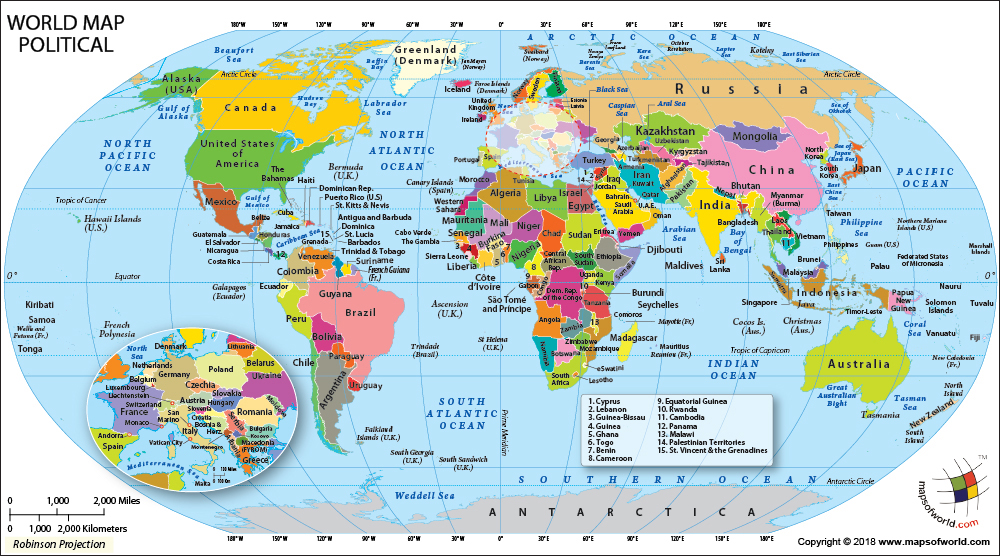
\includegraphics[width=400px]{world-political-map}

\subsection{Take some stuff from R and put it in
text!}\label{take-some-stuff-from-r-and-put-it-in-text}

\begin{Shaded}
\begin{Highlighting}[]
\CommentTok{# in this chunk, I asked the output to be shown with echo=TRUE }
\CommentTok{# Get the maximum value of a product, with function max(). }
\CommentTok{# Need to set na.rm=T because there are NA values in the column.}
\NormalTok{m <-}\StringTok{ }\KeywordTok{max}\NormalTok{(ds$KTonnes,}\DataTypeTok{na.rm=}\NormalTok{T)}

\CommentTok{# Then look up which area has that value for the column KTonnes}
\NormalTok{a <-}\StringTok{ }\NormalTok{ds[ds$KTonnes %in%}\StringTok{ }\NormalTok{m ,]$Area}

\CommentTok{# And which item it is}
\NormalTok{i <-}\StringTok{ }\NormalTok{ds[ds$KTonnes %in%}\StringTok{ }\NormalTok{m ,]$Item}

\CommentTok{# And which year!}
\NormalTok{y <-}\StringTok{ }\NormalTok{ds[ds$KTonnes %in%}\StringTok{ }\NormalTok{m ,]$Year}

\CommentTok{# Then, we can use those values in text by surrounding with `` and prefacing with r}
\end{Highlighting}
\end{Shaded}

The single largest export in a year was from China, mainland in 2013 and
it was 4.89299\times 10\^{}\{8\} tonnes of Vegetables.

\section{The goal for today is to investigate food / feed production
over time by
countries.}\label{the-goal-for-today-is-to-investigate-food-feed-production-over-time-by-countries.}

Summarise some data, plot some data, and find some patterns!

\subsection{Questions to ask:}\label{questions-to-ask}

\begin{itemize}
\tightlist
\item
  Pick a food type and look at where it's grown over time
\item
  Pick a country and find what's been grown in it over time
\item
  Pick a year and see what's been grown where
\item
  Look at differences in food (for people) vs feed (for animals) for a
  country or set of countries
\end{itemize}

\subsection{For advanced R users: Go forth on your own from
here!}\label{for-advanced-r-users-go-forth-on-your-own-from-here}

\subsection{For beginners\ldots{} here are some code chunks to use to
get you
started.}\label{for-beginners-here-are-some-code-chunks-to-use-to-get-you-started.}

\section{Data Sumamrising}\label{data-sumamrising}

\begin{Shaded}
\begin{Highlighting}[]
\CommentTok{# in this chunk, I asked everything to be shown with echo=TRUE }
\CommentTok{# Here are some useful tabulation commands. These use the tidyverse.}
\CommentTok{# This takes data and summarises for output. }
\CommentTok{# %>% is a 'pipe' and passes commands between lines.}

\CommentTok{# you can filter columns. here, we want columns where the item is sugar cane, used for food}
\NormalTok{t2 <-}\StringTok{ }\NormalTok{ds %>%}
\StringTok{  }\KeywordTok{filter}\NormalTok{(Item==}\StringTok{"Sugar cane"}\NormalTok{) %>%}
\StringTok{  }\KeywordTok{filter}\NormalTok{(Element==}\StringTok{"Food"}\NormalTok{)}

\NormalTok{t2}
\end{Highlighting}
\end{Shaded}

\begin{verbatim}
## # A tibble: 2,650 x 13
##    Area.Abbreviation Area.Code Area   Item.Code Item  Element.Code Element
##    <fct>                 <int> <fct>      <int> <fct>        <int> <fct>  
##  1 BGD                      16 Bangl~      2536 Suga~         5142 Food   
##  2 BWA                      20 Botsw~      2536 Suga~         5142 Food   
##  3 BRA                      21 Brazil      2536 Suga~         5142 Food   
##  4 BRN                      26 Brune~      2536 Suga~         5142 Food   
##  5 KHM                     115 Cambo~      2536 Suga~         5142 Food   
##  6 CMR                      32 Camer~      2536 Suga~         5142 Food   
##  7 CHN                      96 China~      2536 Suga~         5142 Food   
##  8 CHN                     128 China~      2536 Suga~         5142 Food   
##  9 CHN                     214 China~      2536 Suga~         5142 Food   
## 10 COD                      46 Congo       2536 Suga~         5142 Food   
## # ... with 2,640 more rows, and 6 more variables: Unit <fct>,
## #   latitude <dbl>, longitude <dbl>, Year <int>, KTonnes <int>, Crop <fct>
\end{verbatim}

\begin{Shaded}
\begin{Highlighting}[]
\CommentTok{# you can use a | operator ('or') to look at multiple selections at once.}
\CommentTok{# you can use the select operator to only show some columns}
\CommentTok{# and the filter operator to remove columns even after summarising}
\CommentTok{# here we ask for only the crops of more than 10*1000 tonnes}
\NormalTok{t3<-}\StringTok{ }\NormalTok{ds %>%}
\StringTok{  }\KeywordTok{filter}\NormalTok{(Area==}\StringTok{"Netherlands"} \NormalTok{|}\StringTok{ }\NormalTok{Area==}\StringTok{"Belgium"}\NormalTok{) %>%}\StringTok{ }
\StringTok{  }\KeywordTok{group_by}\NormalTok{(Area,Crop,Element,Year) %>%}
\StringTok{  }\KeywordTok{summarise}\NormalTok{(}\DataTypeTok{TotalKTonnes =} \KeywordTok{sum}\NormalTok{(}\KeywordTok{as.numeric}\NormalTok{(KTonnes)) ) %>%}
\StringTok{  }\KeywordTok{filter}\NormalTok{(TotalKTonnes >}\StringTok{ }\DecValTok{10}\NormalTok{)}

\NormalTok{t3}
\end{Highlighting}
\end{Shaded}

\begin{verbatim}
## # A tibble: 1,839 x 5
## # Groups:   Area, Crop, Element [62]
##    Area    Crop    Element  Year TotalKTonnes
##    <fct>   <fct>   <fct>   <int>        <dbl>
##  1 Belgium Alcohol Food     2000         2618
##  2 Belgium Alcohol Food     2001         2590
##  3 Belgium Alcohol Food     2002         2512
##  4 Belgium Alcohol Food     2003         2483
##  5 Belgium Alcohol Food     2004         2521
##  6 Belgium Alcohol Food     2005         2722
##  7 Belgium Alcohol Food     2006         2604
##  8 Belgium Alcohol Food     2007         2478
##  9 Belgium Alcohol Food     2008         2416
## 10 Belgium Alcohol Food     2009         2455
## # ... with 1,829 more rows
\end{verbatim}

\begin{Shaded}
\begin{Highlighting}[]
\CommentTok{# We can make lists and use these to filter. }
\CommentTok{# Here's list of some things eaten by people and animals}
\NormalTok{mixed <-}\StringTok{ }\KeywordTok{c}\NormalTok{(}\StringTok{"Oats"}\NormalTok{,}\StringTok{"Soyabeans"}\NormalTok{, }\StringTok{"Sugar cane"}\NormalTok{)}

\CommentTok{# this will generate an error, but it actually works. }
\CommentTok{#an example of tidyverse 'lazy evaluation'}
\NormalTok{t4<-}\StringTok{ }\NormalTok{ds %>%}
\StringTok{  }\KeywordTok{filter}\NormalTok{(Area==}\StringTok{"Brazil"} \NormalTok{|}\StringTok{ }\NormalTok{Area==}\StringTok{"Colombia"}\NormalTok{) %>%}
\StringTok{  }\KeywordTok{filter}\NormalTok{(Item==mixed)}
\end{Highlighting}
\end{Shaded}

\begin{verbatim}
## Warning in is.na(e1) | is.na(e2): longer object length is not a multiple of
## shorter object length
\end{verbatim}

\begin{verbatim}
## Warning in `==.default`(Item, mixed): longer object length is not a
## multiple of shorter object length
\end{verbatim}

\begin{Shaded}
\begin{Highlighting}[]
\NormalTok{t4 }
\end{Highlighting}
\end{Shaded}

\begin{verbatim}
## # A tibble: 143 x 13
##    Area.Abbreviation Area.Code Area  Item.Code Item   Element.Code Element
##    <fct>                 <int> <fct>     <int> <fct>         <int> <fct>  
##  1 BRA                      21 Braz~      2516 Oats           5142 Food   
##  2 BRA                      21 Braz~      2536 Sugar~         5521 Feed   
##  3 BRA                      21 Braz~      2555 Soyab~         5521 Feed   
##  4 COL                      44 Colo~      2555 Soyab~         5142 Food   
##  5 BRA                      21 Braz~      2536 Sugar~         5142 Food   
##  6 BRA                      21 Braz~      2555 Soyab~         5142 Food   
##  7 COL                      44 Colo~      2516 Oats           5142 Food   
##  8 COL                      44 Colo~      2536 Sugar~         5521 Feed   
##  9 BRA                      21 Braz~      2516 Oats           5142 Food   
## 10 BRA                      21 Braz~      2536 Sugar~         5521 Feed   
## # ... with 133 more rows, and 6 more variables: Unit <fct>,
## #   latitude <dbl>, longitude <dbl>, Year <int>, KTonnes <int>, Crop <fct>
\end{verbatim}

\begin{Shaded}
\begin{Highlighting}[]
\CommentTok{# finally, we can put these together to summarise.}
\CommentTok{# Here, we are taking mass of items grown in Brazil or Colombia}
\CommentTok{# and taking together the sum of all tonnes by year across rows}
\CommentTok{# (= total production in these countries, whether for food or feed)}
\CommentTok{# (Note that I used a less lazy evaluaton method here for the filter)}

\NormalTok{t5<-}\StringTok{ }\NormalTok{ds %>%}
\StringTok{  }\KeywordTok{filter}\NormalTok{(Item %in%}\StringTok{ }\NormalTok{mixed ==}\StringTok{ }\NormalTok{T) %>%}
\StringTok{  }\KeywordTok{filter}\NormalTok{(Area==}\StringTok{"Brazil"} \NormalTok{|}\StringTok{ }\NormalTok{Area==}\StringTok{"Colombia"}\NormalTok{) %>%}
\StringTok{  }\KeywordTok{group_by}\NormalTok{(Year,Item) %>%}\StringTok{ }
\StringTok{  }\KeywordTok{summarise}\NormalTok{(}\DataTypeTok{TotalKTonnes =} \KeywordTok{sum}\NormalTok{(}\KeywordTok{as.numeric}\NormalTok{(KTonnes))  ) }

\NormalTok{t5}
\end{Highlighting}
\end{Shaded}

\begin{verbatim}
## # A tibble: 159 x 3
## # Groups:   Year [?]
##     Year Item       TotalKTonnes
##    <int> <fct>             <dbl>
##  1  1961 Oats                 37
##  2  1961 Soyabeans            49
##  3  1961 Sugar cane        11537
##  4  1962 Oats                 36
##  5  1962 Soyabeans            68
##  6  1962 Sugar cane        15738
##  7  1963 Oats                 33
##  8  1963 Soyabeans            84
##  9  1963 Sugar cane        17246
## 10  1964 Oats                 35
## # ... with 149 more rows
\end{verbatim}

\newpage 

\%\%newpage is a command for Latex\ldots{}and \% is the comment
character for Latex. \#\# Plotting

\begin{Shaded}
\begin{Highlighting}[]
\CommentTok{# We can easily plot these with lines, points, and bars!}
\CommentTok{# we are using ggplot here. }
\CommentTok{#The first line sets up what the data are & what values are mapped to things}
\CommentTok{# in the plot ('aes' values).}
\CommentTok{# variables that are useful include: x, y values, color, lty (=line type)}
\CommentTok{# we can then add points or lines or bars with geom_point, geom_line, geom_bar}

\KeywordTok{ggplot}\NormalTok{(}\DataTypeTok{data=}\NormalTok{t5,}\KeywordTok{aes}\NormalTok{(}\DataTypeTok{x=}\NormalTok{Year,}\DataTypeTok{y=}\NormalTok{TotalKTonnes,}\DataTypeTok{color=}\NormalTok{Item))+}
\StringTok{  }\KeywordTok{geom_point}\NormalTok{()}
\end{Highlighting}
\end{Shaded}

\includegraphics{RLadies-GDD_files/figure-latex/unnamed-chunk-10-1.pdf}
\newpage

\begin{Shaded}
\begin{Highlighting}[]
\CommentTok{# add connector lines}
\CommentTok{# and make separate panels with facet_grid }
\CommentTok{#(explore what the ~ does by trying .~Area vs Area~.)}
\KeywordTok{ggplot}\NormalTok{(}\DataTypeTok{data=}\NormalTok{t4,}\KeywordTok{aes}\NormalTok{(}\DataTypeTok{x=}\NormalTok{Year,}\DataTypeTok{y=}\NormalTok{KTonnes,}\DataTypeTok{color=}\NormalTok{Item,}\DataTypeTok{lty=}\NormalTok{Element))+}
\StringTok{  }\KeywordTok{geom_point}\NormalTok{()+}
\StringTok{  }\KeywordTok{geom_line}\NormalTok{()+}
\StringTok{  }\KeywordTok{facet_grid}\NormalTok{(.~Area)}
\end{Highlighting}
\end{Shaded}

\includegraphics{RLadies-GDD_files/figure-latex/unnamed-chunk-11-1.pdf}
\newpage

\begin{Shaded}
\begin{Highlighting}[]
\CommentTok{# Here's an example of a bar plot}
\CommentTok{# And an example of user-specified figure height / width}
\KeywordTok{ggplot}\NormalTok{(}\DataTypeTok{data=}\NormalTok{t3,}\KeywordTok{aes}\NormalTok{(}\DataTypeTok{x=}\NormalTok{Year,}\DataTypeTok{y=}\NormalTok{TotalKTonnes,}\DataTypeTok{fill=}\NormalTok{Crop))+}
\StringTok{  }\KeywordTok{geom_bar}\NormalTok{(}\DataTypeTok{stat=}\StringTok{'identity'}\NormalTok{)+}
\StringTok{  }\KeywordTok{facet_grid}\NormalTok{(Area~.)+}
\StringTok{  }\KeywordTok{theme}\NormalTok{(}\DataTypeTok{legend.position=}\StringTok{"bottom"}\NormalTok{)}
\end{Highlighting}
\end{Shaded}

\includegraphics[width=8000px]{RLadies-GDD_files/figure-latex/unnamed-chunk-12-1}
\newpage

\subsection{Tables of output}\label{tables-of-output}

\begin{Shaded}
\begin{Highlighting}[]
\CommentTok{#Most of what we did earlier was tibbles: }
\CommentTok{#this was a concious choice because the data structures were too big.}
\CommentTok{#Where 'tables' really shine is with summary data.}

\CommentTok{# here, we make a new  variable with 'mutate'-- the last tibble 'verb'}
\NormalTok{t6 <-}\StringTok{ }\NormalTok{ds %>%}
\StringTok{  }\KeywordTok{filter}\NormalTok{(Item %in%}\StringTok{ }\NormalTok{mixed ==}\StringTok{ }\NormalTok{T) %>%}
\StringTok{  }\KeywordTok{filter}\NormalTok{(Area==}\StringTok{"Brazil"} \NormalTok{|}\StringTok{ }\NormalTok{Area==}\StringTok{"Colombia"}\NormalTok{) %>%}
\StringTok{  }\KeywordTok{mutate}\NormalTok{(}\DataTypeTok{Decade=}\KeywordTok{round}\NormalTok{(((Year}\DecValTok{-5}\NormalTok{)/}\DecValTok{10}\NormalTok{),}\DecValTok{0}\NormalTok{)*}\DecValTok{10}\NormalTok{) %>%}\StringTok{  }
\StringTok{  }\CommentTok{# year minus 5, divided by 10, rounded to 0 decimal places.}
\StringTok{  }\CommentTok{# (1969 - 5)/10=196.4, rounds to 1960}
\StringTok{  }\KeywordTok{group_by}\NormalTok{(Decade,Item) %>%}\StringTok{ }
\StringTok{  }\KeywordTok{summarise}\NormalTok{(}\DataTypeTok{TotalKTonnes =} \KeywordTok{sum}\NormalTok{(}\KeywordTok{as.numeric}\NormalTok{(KTonnes))  ) %>%}
\StringTok{  }\KeywordTok{arrange}\NormalTok{(Item,Decade)}

\NormalTok{t6 <-}\StringTok{ }\KeywordTok{as.data.frame}\NormalTok{(t6)}

\KeywordTok{kable}\NormalTok{(t6)}
\end{Highlighting}
\end{Shaded}

\begin{longtable}[]{@{}rlr@{}}
\toprule
Decade & Item & TotalKTonnes\tabularnewline
\midrule
\endhead
1960 & Oats & 404\tabularnewline
1970 & Oats & 628\tabularnewline
1980 & Oats & 1522\tabularnewline
1990 & Oats & 2113\tabularnewline
2000 & Oats & 3665\tabularnewline
2010 & Oats & 1186\tabularnewline
1960 & Soyabeans & 811\tabularnewline
1970 & Soyabeans & 2933\tabularnewline
1980 & Soyabeans & 8913\tabularnewline
1990 & Soyabeans & 9933\tabularnewline
2000 & Soyabeans & 11735\tabularnewline
2010 & Soyabeans & 4026\tabularnewline
1960 & Sugar cane & 140452\tabularnewline
1970 & Sugar cane & 76504\tabularnewline
1980 & Sugar cane & 69605\tabularnewline
1990 & Sugar cane & 43270\tabularnewline
2000 & Sugar cane & 68551\tabularnewline
2010 & Sugar cane & 30526\tabularnewline
\bottomrule
\end{longtable}

\newpage

\begin{Shaded}
\begin{Highlighting}[]
\CommentTok{#We can also restructure the table}
\CommentTok{# this uses matrix notation to paste together elements by column}
\CommentTok{# I've also put the units in tonnes again}
\KeywordTok{kable}\NormalTok{(}\KeywordTok{cbind}\NormalTok{(t6[}\DecValTok{1}\NormalTok{:}\DecValTok{6}\NormalTok{,}\DecValTok{1}\NormalTok{],t6[}\DecValTok{1}\NormalTok{:}\DecValTok{6}\NormalTok{,}\DecValTok{3}\NormalTok{]*}\DecValTok{1000}\NormalTok{,t6[}\DecValTok{7}\NormalTok{:}\DecValTok{12}\NormalTok{,}\DecValTok{3}\NormalTok{]*}\DecValTok{1000}\NormalTok{,t6[}\DecValTok{13}\NormalTok{:}\DecValTok{18}\NormalTok{,}\DecValTok{3}\NormalTok{]*}\DecValTok{1000}\NormalTok{),}
      \DataTypeTok{col.names=}\KeywordTok{c}\NormalTok{(}\StringTok{"Year"}\NormalTok{,}\StringTok{"Tonnes/Oats"}\NormalTok{,}\StringTok{"Tonnes/Soya"}\NormalTok{,}\StringTok{"Tonnes/Sugar Cane"}\NormalTok{))}
\end{Highlighting}
\end{Shaded}

\begin{longtable}[]{@{}rrrr@{}}
\toprule
Year & Tonnes/Oats & Tonnes/Soya & Tonnes/Sugar Cane\tabularnewline
\midrule
\endhead
1960 & 404000 & 811000 & 140452000\tabularnewline
1970 & 628000 & 2933000 & 76504000\tabularnewline
1980 & 1522000 & 8913000 & 69605000\tabularnewline
1990 & 2113000 & 9933000 & 43270000\tabularnewline
2000 & 3665000 & 11735000 & 68551000\tabularnewline
2010 & 1186000 & 4026000 & 30526000\tabularnewline
\bottomrule
\end{longtable}

\subsection{Cool! Adapt these code chunks to ask some questions and make
a nice summary of it with
Markdown.}\label{cool-adapt-these-code-chunks-to-ask-some-questions-and-make-a-nice-summary-of-it-with-markdown.}


\end{document}
